\documentclass[12pt,a4paper]{article}
\setlength{\topmargin}{0.0in}
\setlength{\oddsidemargin}{0.33in}
\setlength{\textheight}{9.0in}
\setlength{\textwidth}{6.0in}
\renewcommand{\baselinestretch}{1.25}

\usepackage[utf8]{inputenc}
\usepackage{amsmath,amsfonts,mathtools,csvsimple,tikz,enumitem}
\usepackage{caption,subcaption}
\usepackage{graphicx}
\usepackage[svgpath=./svgs/]{svg}
\usepackage[extract=true]{svg-extract}
\usepackage{float}
\usepackage[style=numeric,backend=biber]{biblatex}
\usepackage{hyperref}
%\svgpath{{svg/}{svg/}}
\addbibresource{bibliography.bib}

\newcommand{\boxalign}[2][0.97\textwidth]{
 \par\noindent\tikzstyle{mybox} = [draw=black,inner sep=6pt]
 \begin{center}\begin{tikzpicture}
  \node [mybox] (box){%
   \begin{minipage}{#1}{\vspace{-5mm}#2}\end{minipage}
  };
 \end{tikzpicture}\end{center}
}

% to build pdf:
% pdflatex main.tex -> biber main -> pdflatex main.tex

\title{Dynamical Community Detection in Directed Networks}
\author{MMSC Special Topic Report for Networks C5.4}
\date{Candidate number: 1048531}

\newtheorem{theorem1}{Perron-Frobenius Theorem for Regular Matrices}
\newtheorem{theorem2}{Perron-Frobenius Theorem for Nonnegative Matrices}

\begin{document}
\maketitle
\thispagestyle{empty}
\newpage
\setcounter{page}{1}

\section{Introduction}

The identification of community structures within a network is a popular, but relatively young field (COMPARING CLUSTERINGS). The identification of communities within a graph has a plethora of applications in biology, sociology and computer science, where information is often examined in a graph structure (FORTUNATO). The assignment of a particular vertex to a particular community upgrades our understanding of it, while the aggregation of many nodes into a few communities reduces the dimensionality of our analysis (MULTISCALE). On the highest-level, clustering algorithms seek to divide networks into discrete communities where the nodes within a each community are highly similar with respect to some measure and nodes from different communities are highly dissimilar. \medskip

\noindent Particularly interesting is the concept of flow-based community detection. Many networks are constructed from the collection of data relating to some dynamical process, e.g. itineraries on a transport network (REF), the spread of ideas in a citation network (REF AND GET MORE). Hence, the network's topology is highly influenced by the dynamical process which it represents. But it is also possible to turn this concept on its head when we consider that a network's structure may in turn influence a dynamical process which runs over it. It is possible for nodes and communities of nodes to be categorised and ranked based on how they will affect any such dynamical process. The paper \textit{The many facets of community detection in complex networks} thus defines dynamical communities on a network as ``blocks of nodes with different identities that trap the flow and channel it in different directions'' \cite{schaub2017many}. An understanding of how topology will affect flow can then be put to many uses such as optimising the flow on a network in the cases of transport systems (REF WAN GUIMERO), vulnerability analysis by identifying key nodes vital to flow (REF DYNAMICAL IMPORTANCE PAPER) or predicting the movement of trade or passengers (REF ROSVALL, KALZA). For the majority of these flow-based methods the dynamic process being modelled is the probability wave of a random walker as it diffuses with time over a network. This useful abstraction allows network scientists to draw expertise from spectral graph theory, control theory and probability theory to extract all sorts of useful results. \medskip

\noindent A lot of the existing literature on spectral graph theory focuses particular attention on undirected networks, primarily due to the attractiveness of the symmetric adjacency matrix which allows for the derivation of appealing theoretical results and simplifications. For most systems, however, direction is nontrivial and the extension of measures derived for symmetric adjacency matrices is not always obvious (DISCUSS TRANSPORT etc.). Additionally, an exciting new branch of network science is looking at the effects of modelling a random walker on a network without the Markov property by constructing so-called `memory networks' (REF SSL ROSVALL). These memory networks have been show to prouced more accurate results in predictive modelling and less information loss (REFERENCE ROSVALL,SSL). However memory networks are directed even if the original network is not (REF) which further motivates our interest in studying popular network measures in the context of directed networks and asymmetric adjacency matrices. \medskip

\noindent Recent new research has begun to find applications and correlations for control theory's model order reduction methods in network science \cite{schaub2017many}. The paper \cite{schaub2019multiscale} proposes a control theory-based approach to quantifying similarities between nodes in a network with respect to some dynamical process running over them. With this ground-up approach it is possible to rederive popular network science community detection method such as Markov Stability and (GET THIS). The paper proposes a standard similarity measure defined by a weighted bilinear product of two vectors which can be augmemted to suit the need at hand. This project will use continuous and discrete-time similarity measures proposed in this paper to construct similarity matrices which can then be used for graph clustering. \medskip


\noindent The report will be organised as follows: first the relationship between control theory, dynamical systems theory and random walks on a network will be established in Section (REF). Then the methods by which similarity matrices are constructed with relation to these processes will be discussed. Two discrete-time similarity measures, along with one continuous-time similarity measure, are chosen for study in the remainder of the report and explained in greater detail in Section (REF). Though alternative methods exist such as Louvain-like combinatorial optimisation \cite{schaub2019multiscale}, spectral methods will be used to perform clustering based on these similarity measures and this will be briefly discussed in Section (REF). In Section (REF) the results of a applying these measures to a simple model network with clear dynamical substructures will be explored. In Section (REF) a similar method will be applied to an airline network extracted from a real world dataset (REF). In Section (REF) a different method of clustering, core-periphery detection, will be discussed and applied to this same airline network. (MEMORY NETWORKS)

\section{Flow on a network}
When a graph is representative of some dynamical system, i.e. a network of roads, a social network, or in a more abstract sense, the flow of information through a citation network, it makes to consider how the the topological structure of a network might affect a process flowing over it. The standard way to study this is to consider injecting a random walker into the network at some time point $t=0$. Analogous to the heat equation in dynamical systems theory, the probability wave for the random walker spreads diffusively throughout the graph, influenced only by structural characteristics such as link availability and weighting. In first-order networks, this random walker is assumed to have the Markov property, and its past trajectory will not affect its subsequent step. Dynamical community detection seeks to identify communities of nodes based on similarities with respect to how they affect the flow of such a walker. Nodes clusters may be compared based on their ability to `trap' a walker for a longer period time, or perhaps based on how a walker will behave in the network after it passes through them. \\

\section{Notation}
Throughout this project we will use the following notation repeatedly:
\begin{itemize}[label=$\cdot$,nosep]
  \item $v_i$ : a specific node on the network
  \item $N$ : the number  of nodes in the network
  \item $y \in \mathbb{R}^{N \times 1}$ : column vector relating to some dynamical process on the network
  \item $p \in \mathbb{R}^{1\times N}$ : row vector of probability densities for the (continuous or discrete-time) Markov process
  \item $\pi \in \mathbb{R}^{1\times N}$ : stationary probability (row) vector for the Markov process
  \item $M_{\vec i}$ : the $i^{\text{th}}$ row of some matrix $M$.
\end{itemize}

\subsubsection{Random walks} \label{section:random walks}
\noindent When a walker is at a node $v_i$, the set of its transition (jump) probabilities out of that node form a vector. Considering an ensemble of walkers moving across the network in synchrony, the collection of these vectors forms a transition matrix for the Markov process $T$ \cite{lambiottenotes}. For a directed, weighted network the form of this is derived from the network structure where $T_{ij} = A_{ij}/s_i^{\text{out}}$. So $A_{ij}$ is the weighting of the link from $v_i$ to $v_j$, and $s_i^{\text{out}}$ is the total outward node strength of $v_i$. For a discrete time random walk (DTRW) the evolution of the process is described by the equation \begin{equation}p^{n+1} = p^n T\end{equation} where $p$ is the row vector of probability densities listed above. \\ \\

\noindent In discrete time, successive jumps by the walkers form a Markov chain which reaches stationarity once a probability distribution $p=\pi$ is reached, i.e. further jumps do not change the probability distibribution for the walkers on the network, i.e.
\begin{equation}\label{eq:stationary}
  \pi = \pi T.
\end{equation}
Here, $\pi$ and $p \in \mathbb{R}^{1\times N}$ are row vectors as this is conventional when representing diffusion processes \cite{schaub2019multiscale}. \medskip

\noindent Because transition matrices are stochastic matrices and all rows sum to unity, we have $T1=1$ and hence the $\lambda_1=1$ is an eigenvalue so the corresponding left eigenvector represents the stationary distribution and can be denoted $\pi$ (\ref{eq:stationary}). Intuitively, once a system has reached equilibrium, further transitions $T$ will not affect the probability distribution over the system. \medskip

\noindent The Perron-Frobenius theorem guarantees that the absolute value of the largest eigenvalue $\lambda_1$ of an asymmetric, primitive matrix (in this case $\lambda_1 = 1$) is unique and that the corresponding positive left and right eigenvectors are unique. This result is guaranteed when the dynamics of the process are ergodic which is guaranteed if, and only if, the the graph consists of a single strongly connected component (SCC). Thus the Perron-Frobenius theorem allows us to find the unique stationary probability distribution of a strongly connected network by simply calculating the left eigenvector associated with the network's dominant eigenvalue \cite{salnikov2016}.

\noindent Further to this, the random walk Laplacian $L_{\text{rw}}= D^{-1}L = I - T$ can be derived and used in the  master equation of a node-centric continuous-time random walk \cite{lambiottenotes}
\begin{equation}
  \dot{p} = -pL_{\text{rw}} = -p (I-T).
\end{equation}
The node-centric random walk has independent identically distributed inter-event times following a Poisson distribution $\sim \text{Poi}(\lambda)$. The parameter $\lambda$ sets the time-scale and so can be normalised to unity without loss of generality \cite{lambiottenotes}. It can be shown that walks defined by the node-centric CTRW are statistically the same as those defined by the DTRW \cite{lambiottenotes}. Additionally, by setting $\dot{p}=0$ it becomes clear that the formula for the stationary distribution is the same as that for the DTRW (\ref{eq:stationary}) \cite{lambiottenotes}.\medskip

\noindent The ergodicity assumption required for the Perron-Frobenius theorem mentioned above to hold often fails in empirical directed networks \cite{lambiottenotes}. Multiple techniques exist in the literature \cite{rosvall2014memory,salnikov2016} to allow us to make use of the Perron-Frobenius theorem in nonergodic systems and we will discuss solutions to this below in the next section.

\section{Synthesising ergodic dynamics}\label{section:ergodic}
By the Perron-Frobenius theorem (see Appendix section \ref{section:theorems}), the assumption of a unique stationary distribution for the random walk process as described above only holds for a process with for ergodic dynamics. Ergodic dynamics are only guaranteed if a network is composed of a single, strongly connected component \cite{lambiottenotes}. Dynamics on directed, real-world networks rarely satisfy this criterion. Also, if a network contains nodes with no out-links (dangling nodes) then the transition matrix will be ill-defined and the the probability density will become asymptotically concentrated on those nodes. \medskip

\noindent In order to be able to make use of measures such as the stationary probability distribution and transition matrices, network scientists make small adjustments to the network in order to make dynamics ergodic. The most popular methods include extracting a strongly connected component from the graph \cite{salnikov2016} and performing all analysis on that, or else intoducing a small amount of \textit{teleportation} to the process \cite{salnikov2016,lambiottenotes,lambiotte2012ranking}. Neither method is perfect; extracting a single connected component is only appropriate if the majority of nodes in a network already belong to a single strongly connected component and not much information is being lost. Alternatively, introducing teleportation can water-down network structures, reduce overclustering (which is desired in community detection) and lead to resolution limits \cite{schaub2019multiscale}. These effects can reduce the effectiveness of popular methods such as Markov stability. Nonetheless, in the case of networks that are not mostly comprised of a single strongly connected component, it remains a good option. \medskip

\noindent A random walk with teleportation is defined on a network as follows: a walker now continues to move along paths defined by the transition matrix with probability $\alpha$ but also may teleport to any node in the network with probability $(1-\alpha )$. The only exception is that when a walker lands on a node with no out-links, it then must teleport with probability unity \cite{lambiottenotes}. This preserves the $T$ matrix's stochasticity so we are still guaranteed an eigenvalue and eigenvector of unity. Thus rate equation for the process becomes
\begin{equation}
p_i(t+1) = \alpha \sum\limits_j p_j(t)T_{ji} + (1-\alpha)u_i, \qquad \alpha \in [0,1].
\end{equation}

\noindent Here $u\in\mathbb{R}^{1\times N}$ is some \textit{preference} row vector representing how likely a walker is to teleport to each node in the network. This leads to a new formal definition of the stationary probability density (known as the PageRank) and the transition matrix \cite{lambiottenotes}:
\begin{align}
  \pi &= \alpha \pi T +(1-\alpha)u \\ \pi &= (1-\alpha)u(I-\alpha T)^{-1} \\
\implies  (T_{\text{teleport}})_{\vec{i}} &= \begin{cases} (1-\alpha)T_{\vec{i}} + \alpha u \quad \text{if } k_i >0 \\ u \qquad \text{if } k_i =0 \end{cases}
\end{align}\label{eq:teleportation}

\noindent Originally, the teleportation vector used, $u$, was a vector of uniform probabilites $( \frac{1}{N} \dots \frac{1}{N})$. More recent papers \ref{lambiottenotes,lambiotte2012ranking}, inspired by the observed correlation between a node's PageRank score and its in-strength have shown that defining $u$ based on the in-strength of each vertex reduces the noise that is injected to the network by teleportation. This is called \textit{smart} teleportation and
$u \coloneqq \begin{pmatrix} \frac{s^{in}_1}{S^{in}} \dots \frac{s^{\text{in}}_N}{S^{\text{in}}} \end{pmatrix} $ where $S = \sum\limits_{j=1}^N s^{\text{in}}_j$. \medskip

\noindent For this analysis, we opt for the teleportation option as described above. All measures calculated in this study will be based on the modified stationary probability distribution and transition matrix as described in Equations (\ref{eq:teleportation}). This has the

\section{Dynamical processes on a network}\label{section:dynamical processes}
An interesting perspective is to consider the movement of a random walker on a network in the context of linear systems and control theory as discussed in \cite{schaub2019multiscale}. Starting by defining a system of very general linear processes, along with methods of quantifying their similarity, we can then extend this understanding to different aspects of continuous and discrete-time random walks \cite{schaub2019multiscale}. Consider the system
\begin{equation}
\dot y(t) = \mathcal{A} y(t),
\label{eq:dynamical systems}
\end{equation}
\noindent where the vector $y_i (t) \in \mathbb R^n$ is a column vector representing the state of a process on the the network at node $v_i$ and time $t$. This is a simplified version of the dynamical process given in \cite{schaub2019multiscale} where $y_i(t)$ is the impulse response of a node in a system to some input, which is omitted from the equation here for simplicity. For the set of vectors $y_i(t)$, this generalised dynamical process has the solution $y_i(t)=\exp (\mathcal A t)y_i(0) $ or in the discrete sense $y_i(t)=\mathcal A^t y_i(0)$. By specifying $\mathcal A$ we may gain insight into the similarity between nodes with relation to various processes which may run over the network structure. \medskip\

\noindent We can assess the similarity of two vectors $\{ y_i(t),y_j(t) \}$ by computing their bilinear product $\psi_{ij}(t) = \langle y_i(t),y_j(t) \rangle $ \cite{schaub2019multiscale}. If the process is behaving similarly on nodes $v_i$ and $v_j$ at time $t$ then it makes sense that this product will be large (Fig \ref{fig:similarity vectors}).

\begin{figure}[H]
    \centering
    \begin{subfigure}[b]{0.4\linewidth}
        \centering
        \begin{tikzpicture}
        \draw[->] (0,0)--(2,3) node[above]{$y_1(t)$};
        \draw[->] (0,0)--(2.5,2) node[right]{$y_2(t)$};
        \end{tikzpicture}
        \caption{$y_1$ and $y_2$ highly similar}
    \end{subfigure}
    \hfill
    \begin{subfigure}[b]{0.4\linewidth}
        \centering
        \begin{tikzpicture}
        \draw[->] (5,1)--(2+4,3) node[above]{$y_1(t)$};
        \draw[->] (5,1)--(2+4,0) node[right]{$y_2(t)$};
        \end{tikzpicture}
        \caption{$y_1$ and $y_2$ not not very similar}
    \end{subfigure}
    \caption{} \label{fig:similarity vectors}
\end{figure}


\noindent A weighting $\mathcal W$ can be added to this measure by computing $\psi_{ij}(t) = \langle y_i(t),y_j(t) \rangle_{\mathcal W} = y_i^\top\mathcal W y_j$. This weighting is often referred to as a null-model \cite{schaub2019multiscale} and can be used to project away uninformative dimensions depending on what information we are trying to extract.  Gathering the $n$ column vectors $\{y_i(t)\}$ in $\mathbb{R}^n$ we form the $n \times n$ matrix $Y(t) = \begin{pmatrix}y_1 & \dots & y_m \end{pmatrix}$ and thus the dynamical similarity matrix for a process (\ref{eq:dynamical systems}) is given by $\Psi(t) = Y^\top \mathcal W Y$. This similarity matrix also has a corresponding distance matrix defined by the Euclidean norm \cite{schaub2019multiscale} as
\begin{equation*}
D_{ij}(t) = ||\mathcal W^{-\frac{1}{2}}(y_i(t) - y_j(t)||_2.
\end{equation*}

\noindent For the case of random walks, the impulse response of interest is the time-evolving probability density function for a random walk on the network as described in Section \ref{section:random walks}. For a discrete-time random walk (DTRW), $p(t)$ is given by the rate equation
\begin{align}
  p(t+1) &= p(t)T \\
  p(t) &= p(0)T^t.
\end{align}
This can be related back to the solution of the discrete form of the system (\ref{eq:dynamical systems}) by taking the transpose of the process. Then $\mathcal A = T^\top$ and the unweighted similarity matrix $\Psi_{\text{DTRW}}=\langle T^\top,T^\top \rangle = T T^\top$. In this case, we assume both processes begin at the same constant (ASSUMPTION) $y^0 = p(0)^\top$ so this will not affect the similarity of the vectors (CHECK). \medskip\

\noindent Likewise, as described in Section \ref{section:random walks}, evolution of node-centric continuous random walk's probabilities are given by $\dot{p} = p(0)\exp(-L_{\text{rw}} t)$. Taking the transpose of this we recover the continuous form of the dynamical process \ref{eq:dynamical systems} with $\mathcal A = -L_{\text{rw}^\top}$. Thus we have a framework to derive continuous or discrete time dynamical similarity measures as follows: for the DTRW
\boxalign{\begin{align}
    y^{n+1} &= T^\top y^n \label{eq:DTRW}\\
  y^{n} &= [T^n]^\top y^0 \notag \\
  \Psi^n &= T^n [T^n]^\top \notag
\end{align}}


\noindent and for the CTRW the set-up is:
\boxalign{\begin{align}
  \dot y(t) &= -L_{\text{rw}}^\top y  \label{eq:CTRW}\\
  y(t) &= e^{-L_{\text{rw}}^\top t}y_0  \notag \\
  \Psi(t) &= e^{-L_{\text{rw}} t} e^{-L_{\text{rw}}^\top t}. \notag
\end{align}}
These methods will be modified by the inclusion of various weightings models $\mathcal W$ to the bilinear product.

% NEW SECTION: SPECIFIC SIMILARITY MEASURES
\section{Specific similarity measures}
The broad system description given above allows us to define time-dependent similarity matrices based on different properties of the flow. We will focus on three in particular,

% SUBSECTION: UNWEIGHTED DISCRETE
\subsubsection{Discrete-time unweighted similarity matrix} \label{sec:DTRW similarity matrix}
Following an example in \cite{schaub2019multiscale} and considering a DTRW on the network as defined in \ref{eq:DTRW} (CHECK CORRECT REF); we construct simple, unweighted similarity matrices $\Psi^n = T^n [T^n] ^\top$ where $n$ represents timesteps. The $i^{\text{th}}$ row of $T^n$ represents the transition probability vector of the a walker originating at $v_i$ after $n$ steps. Thus, nodes $v_i$ and $v_j$ are said to be similar if their transition probability vectors after $n$ steps are similar, i.e. the $i^{\text{th}}$ and $j^{\text{th}}$ rows of $T^n$ are similar. This is equivalent to stating that two discrete-time random walkers tend to fall upon similar trajectories after leaving nodes $v_i$ and $v_j$.
(CHECK ABOUT STATIONARITY INITIAL CONDITION)

% NEW SUBSECTION: SIMILARITY MATRIX FOR WALKTRAP
\subsubsection{Walktrap-like similarity matrix} \label{sec:Walktrap similarity matrix}
In the Walktrap algorithm, proposed in 2005 by Pascal Pons and Matthieu Latapy \cite{pons2006walktrap}, two nodes $v_i$ and $v_j$ are viewed as similar if DTRW walkers are likely to follow similar trajectories in $n$ steps once they leave those nodes \cite{lambiottenotes}. Again, this is represented by the $i^{\text{th}}$ and $j^{\text{th}}$ rows of $T^n$. The Walktrap measure augments the previous similarity matrix by including a null model which discounts the effect of the equilibrium probability distribution on these probabilities.  \medskip
\noindent Hence, nodes are classed as similar in time $n$ if walkers which originate from them have similar probability distributions over the network after $n$ steps \cite{pons,lecs}. In the original paper, the algorithm is defined for an undirected network with respect to the Euclidean distance between any two nodes transition probability vectors $T_{\vec{i}}^n$ and $T_{\vec{j}}^n$ as
\begin{equation}
  r_{ij} = ||D^{-1/2}(T_{i \bar \ell}^n - T_{j \bar \ell}^n)||_2
\end{equation}

\noindent Here, $n$ should be chosen sufficiently large for a node to be able to traverse the entire network in $n$ steps but not so large that both vectors $T_{\vec{i}}^n$ and $T_{\vec{j}}^n$ start approaching the stationary distribution of the network \cite{lambiottenotes} in which case they will become completely similar. The weighting matrix for the undirected network, which is a diagonal matrix of its stationary distribution $D^{-1} = \text{diag}(\frac{1}{k_1} \dots \frac{1}{k_n}$ represents the probability of a walker visiting each node at equilibrium, regardless of its origin. In the directed case this probability is given by the diagonal matrix of the stationary distribution $\Pi \coloneqq \text{diag}(\pi)$. In the case of non-ergodic dynamics $\pi$  and $T$ are defined to include teleportation as described in \ref{section:ergodic}. As described in Section \ref{section:dynamical processes}, this translates to a similarity matrix.
\begin{equation}
    \Psi_{\Pi}^n = T^n \Pi [T^n]^\top .
\end{equation}

\subsubsection{Continuous-time dynamical similarity matrix} \label{sec:CTRW similarity matrix}
We also examine a dynamical similarity based on the CTRW, similar to work by \cite{schaub2019multiscale}. Here we use the continuous version of the system \ref{eq:dynamical systems} which yields \ref{eq:CTRW} to describe dynamical similarity between nodes $v_i$ and $v_j$ at time $t$. This can be considered like continuous analog of the previous similarity measures. Using the null model as derived in \cite{schaub2019multiscale} $\mathcal W = \Pi - \pi^\top \pi$, where $\Pi = \text{diag}()\pi$ and the second term forms a rank-1 matrix since $\pi$ is a row vector, the similarity matrix becomes
\begin{equation}
  \Psi_{\mathcal W}(t) = e^{-L_{\text{rw}t}}\mathcal{W}e^{-L_{\text{rw}\top t}}.
\end{equation} (CHECK ASSUMPTION) This weighting matrix will produce negative values in our similarity matrix, but since similarity is considered a directionless quantity we justify taking the absolute values of all elements in $\Psi_{\mathcal W}$.

\subsection{Practical considerations}
\subsubsection{Time-scales}
Results obtained will differ depending on the time-scales used. Short time-scales will only identify local communities as walkers do not have time to explore the whole network. If time-scales are too long, however, the Markov process will approach its stationary distribution and the probability distributions of paths originating from all the nodes appear too similar to differentiate. Also for a network that isn't fully-connected it may not be possible for a walker to traverse between any two nodes in finite time. This is largely mitigated here through the inclusion of teleportation.Visualising the similarity matrices, as shown in the sections below, will give an indication as to at what point the stationary distribution begins to mask structure in the network. For this project, inspection of heatmaps of the similarity matrices will be used to estimate appropriate time-scales.

\subsubsection{Comment on normalising similarity matrices}
Since all elements of the transition matrices for the DTRW are probabilities, all elements are within $[0,1]$. By row-stochasticity of $T$ have the same $||\cdot||_1$-norm but vectors with larger $||\cdot||_2$-norms may appear disproportionately similar. To address this, we normalise all row vectors with respect to their 2-norms before taking the bilinear product. In the weighted case, the weighting is on the same scale as the original vectors, so the weighting is applied before normalising as follows
\begin{align*}
  \tilde \Psi_{ij} = \frac{y_i^\top \mathcal W y_j} {||\mathcal W^{1/2} y_i||_2 ||\mathcal W^{1/2} y_i||_2},
\end{align*}
Thus this product will have value unity if the vectors are identical. (ELABORATE IN APPENDIX AND COMPARE SOLUTIONS TO UNWEIGHTED CASE).

\subsubsection{Similarity-based clustering}\label{section:spectral clustering}
Once the similarity matrices have been constructed, they can be used to cluster the network into separate dynamical modules. This can be achieved by Louvain-like block detection or spectral clustering \cite{schaub2019multiscale}. This project will use the \texttt{SpectralClustering()} function provided in Python's sklearn module \cite{scikit-learn} for this purpose. \medskip
\noindent To give a brief overview of the methodology, spectral clustering methods work as follows \cite{lambiottenotes,schaub2019multiscale,Luxburg07atutorial}: the first $c$ eigenvectors corresponding the the dominant $c$ eigenvalues of the similarity matrix $\Psi(t)$ are assembled, forming a new matrix $U \in \mathbb{R}^{N \times c}$. Letting the $N$ vectors $ \{ y_i \in \mathbb{R}^c \} $, be the row vectors of this $U$, $k$-means clustering is then applied to assign each $y_i$ to one of $k$ clusters $\mathcal C_1,...,\mathcal C_k $. As is common practise, the \texttt{SpectralClustering()} function defaults to considering the same number of eigenvectors as clusters requested, $c=k$. This method has the disadvantage that it requires the user to specify the desired number of clusters in advance so cluster numbers will be entered manually, based on qualitative inspection of similarity matrices and what information is being considered.

% NEW SECTION: MODEL NETWORK
\section{Initial analysis on a model network}\label{section:model network}
We will now perform a qualitative assessment of these similarity measures in the context of a model network that has an obvious dynamical structure. We look at a network originally presented in the paper \cite{schaub2019multiscale}. This network's setup and adjacency matrix is shown in Figure \ref{fig:toy net adjacency matrix}.  The network is directed, not strongly connected \cite{schaub2019multiscale} and contains a bipartite substructure between the nodes $\{5,6,7,8\}$ and $\{ 9,10,11 \}$ while the nodes $\{ 1,2,3,4 \}$ have a cyclic substructure and walkers which leave this substructure cannot return. Thus the probability of a walker inhabiting that segment of the network may only decrease with time. Edge weightings are not listed in the paper so estimates are made based on the visuals provided. This network's multiple dynamical substructures make it a good model with which to highlight the effects that different similarity measures emphasise. \medskip

\noindent Clusterings are selected using spectral clustering on the similarity matrices as discussed in Section \ref{section:spectral clustering}. The results of performing clustering on these matrices at time $t=20$ are shown at the bottom of this section in Figure \ref{fig:toy net predictions t20}.

\begin{figure}[H]
\centering
\begin{subfigure}[b]{0.35\linewidth}
  \centering
  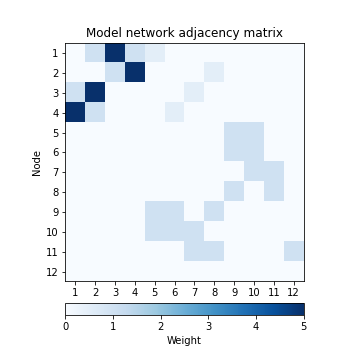
\includegraphics[width=\textwidth]{toy_net/toy net adjacency matrix.png}
  \caption{}
  \label{fig:toy net diagram}
\end{subfigure}
\hfill
\begin{subfigure}[b]{0.5\linewidth}
  \centering
  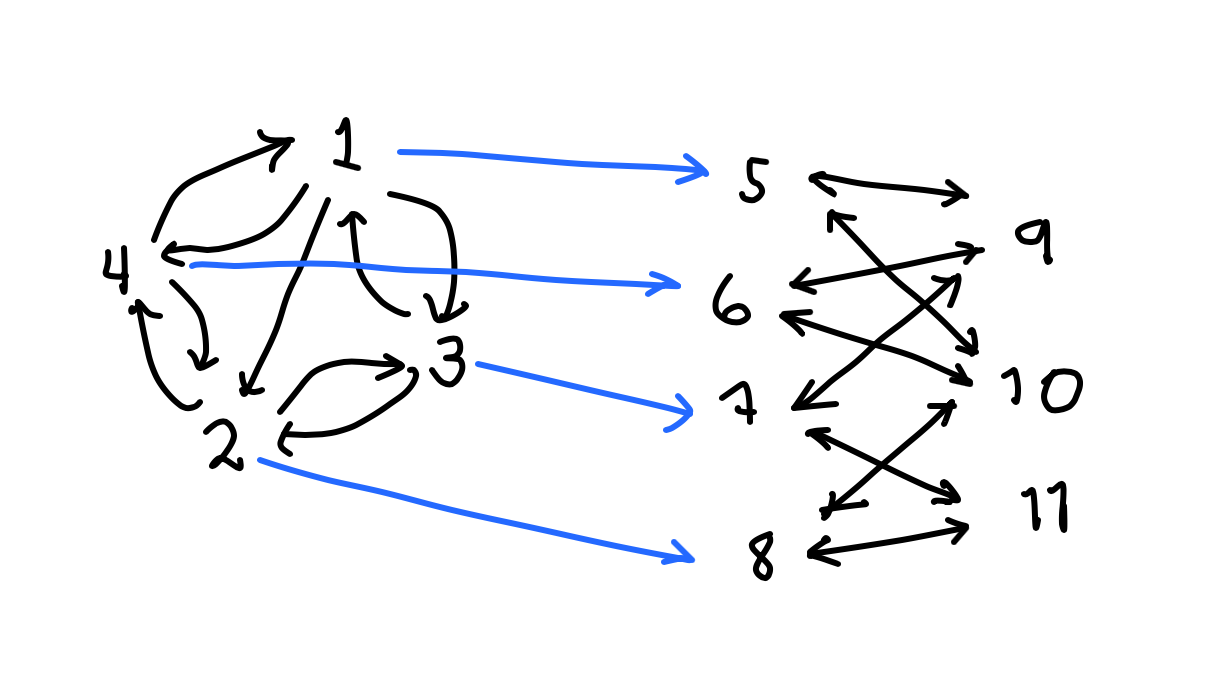
\includegraphics[width=\textwidth]{toy_net/toy_net_diagram.png}
  \caption{}
  \label{fig:toy net adjacency matrix}
\end{subfigure}
\caption{Adjacency matrix for model network in \cite{schaub2019multiscale}.}
\label{fig:toy net}
\end{figure}

\subsubsection{Unweighted DTRW performance}
The original paper \cite{schaub2019multiscale} looked at the unweighted similarity matrix \ref{sec:DTRW similarity matrix} for a DTRW on the network using \ref{eq:DTRW}. This similarity matrix is shown in Figure \ref{fig:DTRW toy sim} where the lighter sections indicate blocks of similar nodes. To begin, we visually inspect these matrices. At time $t=2$ the network appears to have $4$ major similar dynamical block $\{1,2\}$, $\{3,4\}$, $\{5,6,7,8\}$ and $\{9,10,11\}$ with a substructure of $\{ 5,6 \}$ and $\{7,8\}$ in $\{5,6,7,8\}$. As time increases the $\{1,2\}$ and $\{3,4\}$ become more similar and blend into one and the more robust three cluster formation becomes dominant.

\begin{figure}[H]
    \centering
    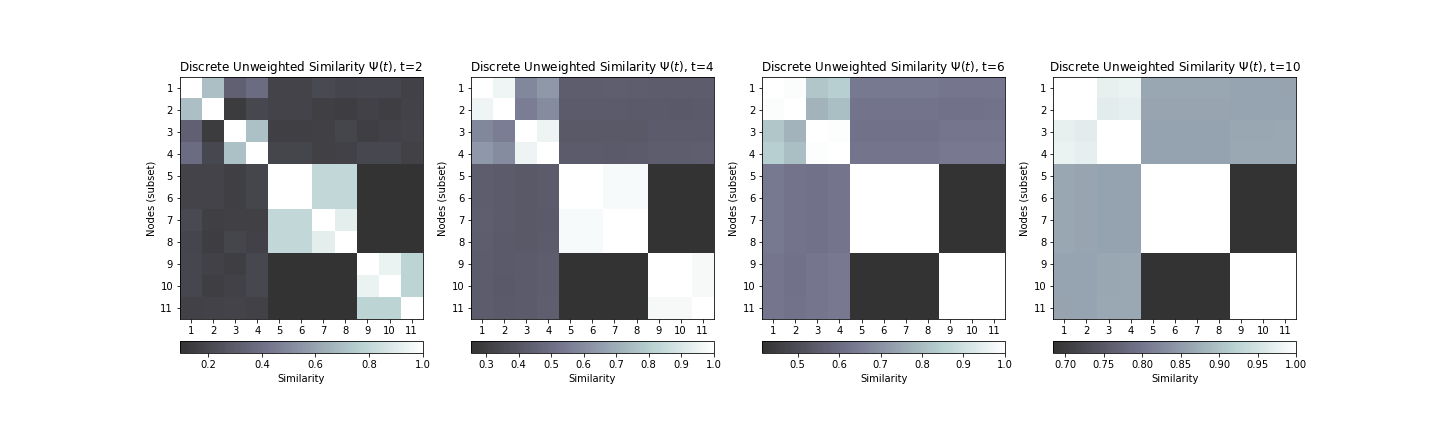
\includegraphics[width=\textwidth]{toy_net/DTRWu_Similarity_toy_net.png}
    \caption{Unweighted DTRW similarity calculated from the bilinear product $ T^n [T^n]^\top$ and normalised with respect to the product of the norms $||T_i^\top||_2 $, $||T_j^\top||_2$.}
    \label{fig:DTRW toy sim}
\end{figure}

\noindent The result of spectral clustering on this matrix is shown by the colour-coded network visualisation in Figure \ref{fig:DTRW t20k3}. This simple similarity measure performs well on the model network and consistently isolates the three clusters $\{ 1,2, 3,4\}$, $\{ 5,6,7,8\}$ and $\{ 9,10,11\}$ even for large time $t \sim 100$. When asked for a only two clusters, the algorithm isolates $\{ 5,6,7,8\}$ from the rest of the network. Nodes in the rest of the network could be considered similar in that they have some probability of entering the $\{ 5,6,7,8\}$ group but nodes in $\{ 5,6,7,8\}$ can only travel between that group and $\{ 9,10,11\}$. When asked for three clusters the algorithm separates the remaining network into $\{ 1,2,3,4\}$ and $\{ 9,10,11\}$.

\subsubsection{Walktrap}
Next, the Walktrap similarity matrix $\Psi_{\text{Walktrap}}$ is calculated for the network by the inclusion of a null model as described in section \ref{sec:Walktrap similarity matrix}. As the network is not ergodic, we use the PageRank for $\pi$ \ref{section:ergodic} instead of the stationary probability distribution and as usual, let $\mathcal W = \text{diag}(\pi)$. The similarity matrix generated is shown in Figure \ref{fig:Walktrap toy sim}. The matrix appears virtually identical to the unweighted similarity matrix. This implies any differences between the two similarity matrices are in scaling-only. (UNSCALED IN APPENDIX). As expected, the results of spectral clustering are identical to those of the unweighted similarity matrix.
\begin{figure}[H]
    \centering
    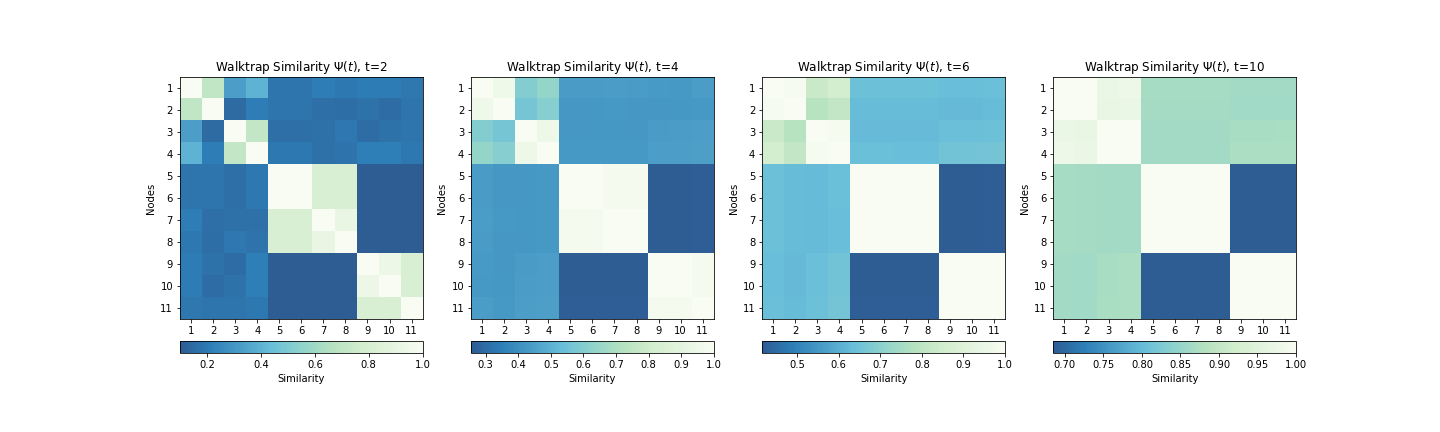
\includegraphics[width=\textwidth]{toy_net/Walktrap_Similarity_toy_net.png}
    \caption{Walktrap similarity using the null model $\mathcal W = \Pi = \text{diag}(\pi)$ where $\pi$ is the PageRank of the network. Calculated from the weighted bilinear product $\langle T^n,T^n \rangle_{\mathcal W}$ and normalised with respect to the product of the norms $||\mathcal{W}^{1/2}T_i^\top||_2$, $|| \mathcal{W}^{1/2}T_j^\top||_2$.}
    \label{fig:Walktrap toy sim}
\end{figure}

\subsection{Dynamical Similarity}
Finally, the dynamical similarity matrix $\Psi_{\text{dynamical}}$ is calculated as in \ref{sec:CTRW similarity matrix} for times $\{ 1,2,6,10 \}$ . As can be seen in Figure \ref{fig:dynamical similarity matrix toy}, dynamical similarity isolates slightly different blocks to the previous two DTRW-based similarity matrices. Sub-clusters in the bi-parite network are visible for small time $t=2$ but by $t=5$ these have blended into one large sub-block representing the entire bi-partite network as one dynamical region. Spectral clustering is performed and the results for time $t=20$ are shown in \ref{fig:dynsim t20k3} When the algorithm is asked for $k=3$ clusters it isolates node $6$ which seems inaccurate. The reason for this becomes clear upon referring back to the similarity matrices and also highlights the disadvantages of a requiring user-specified number of clusters. The similarity matrix has clearly identified only two blocks so requesting $k\geq3$ clusters will require it to look for extremely dissimilarities on a very small scale, possibly down to machine precision at which point dissimilarities are random and informative. Indeed, for $k=20$ all entries in the lower-right block of $\Psi$ are identically one. \medskip

\noindent When asked for $k=2$ clusters the algorithm effectively differentiates the bipartite substructure from the reat of the network (PUT IN APPENDIX?).
\begin{figure}[H]
    \centering
    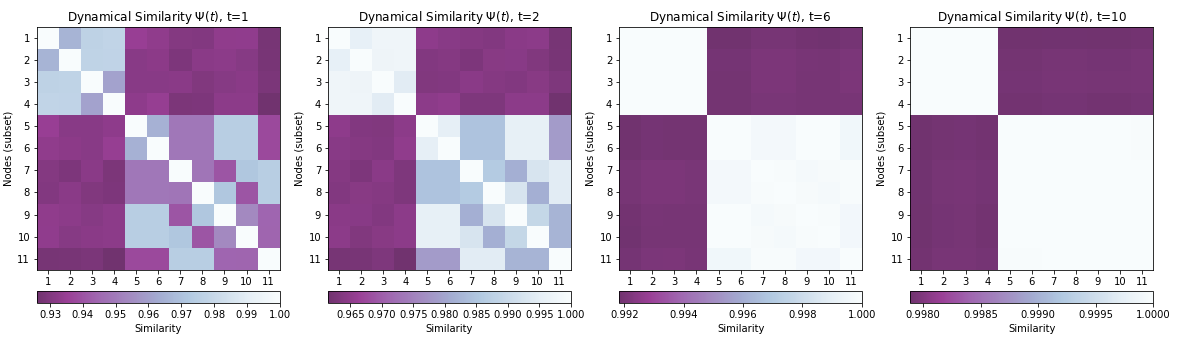
\includegraphics[width=\textwidth]{toy_net/Dynamical_Similarity_toy_net.png}
    \caption{CTRW dynamical similarity matrix of the model network using the null model $\mathcal W = \Pi - \pi \pi^\top $ where $\pi$ is the PageRank of the network. Calculated as described in Section \ref{sec:CTRW similarity matrix}.}
    \label{fig:dynamical similarity matrix toy}
\end{figure}

\begin{figure}[H]
  \begin{subfigure}[b]{0.3\textwidth}
    \centering
    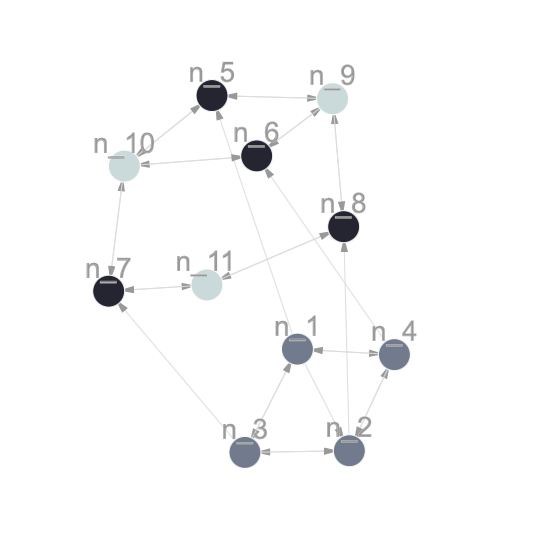
\includegraphics[width=\textwidth]{toy_net/unweighted t20.png}
    \caption{}
    \label{fig:DTRW t20k3}
  \end{subfigure}
  \hfill
  \begin{subfigure}[b]{0.3\textwidth}
    \centering
    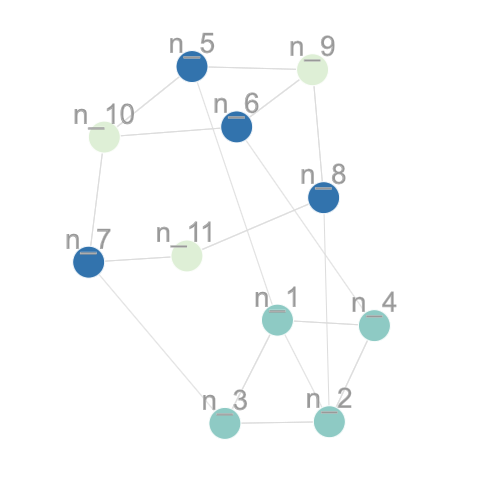
\includegraphics[width=\textwidth]{toy_net/walktrap t20.png}
    \caption{}
    \label{fig:wt t20k3}
  \end{subfigure}
  \hfill
  \begin{subfigure}[b]{0.3\textwidth}
    \centering
    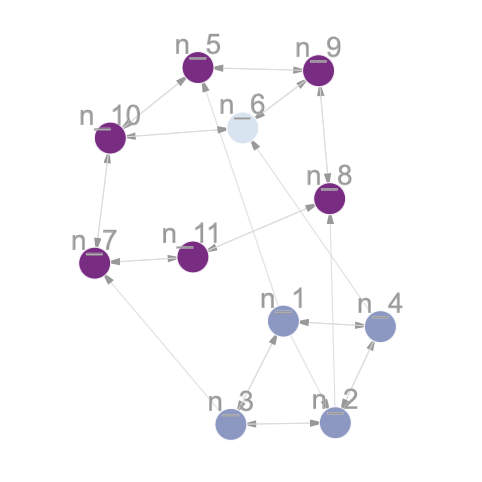
\includegraphics[width=\textwidth]{toy_net/dynamical similarity t20.png}
    \caption{}
    \label{fig:dynsim t20k3}
  \end{subfigure}
  \caption{}
  \label{fig:toy net predictions t20}
\end{figure}

% SECTION: FLIGHT NETWORK
\section{Flight Network}
We now consider the performance of these measures on a real world flight network. The first dataset is a set of passenger itineraries from the first quarter of 2011 and consists of flights to and from 103 Californian airports. The network contains 474 edges \cite{flightdata}. The network's adjacency matrix, shown Figure \ref{fig:flights adjacency matrix} is suggestive of some core-peripheral structure in the network. The presence of core-peripheral structures in airline networks is well-documented (REFERENCE AND EXPLAIN). The normalised similarity measures for discrete dynamical, Walktrap and continuous dynamical similarity are all shown in Figures \ref{fig:DTRW flights}, \ref{fig:Walktrap flights} and \ref{fig:dynamical similarity matrix flights}.

\begin{figure}[H]
  \centering
  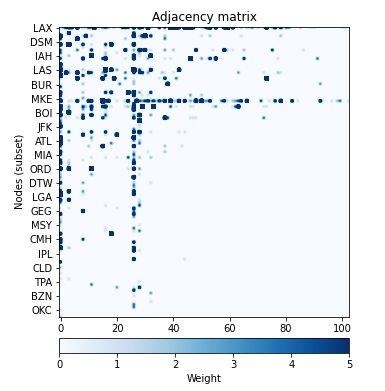
\includegraphics[width=0.4\textwidth]{flight_net/flights adjacency.png}
  \caption{Heatmap of the weighted adjacency matrix for the flights network \cite{flightdata} with a subset of nodes listed on the y-axes.}
  \label{fig:flights adjacency matrix}
\end{figure}
\begin{figure}[H]
    \centering
    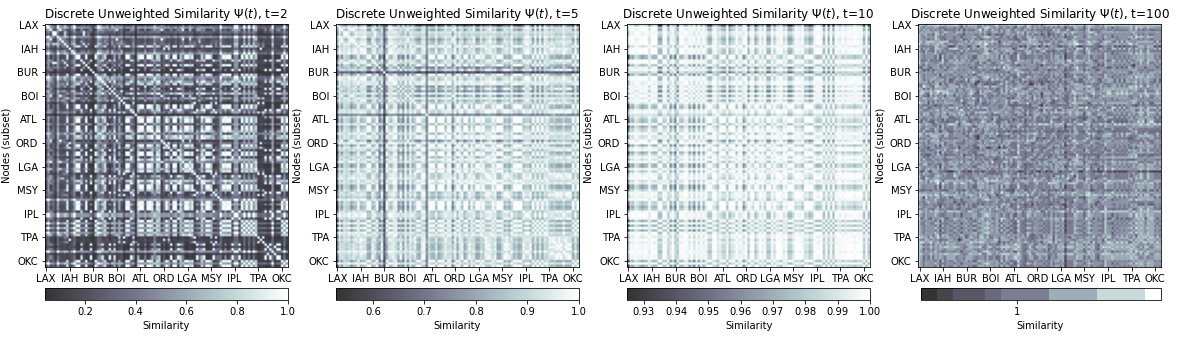
\includegraphics[width=\textwidth]{flight_net/DTRWu_Similarity_flights.png}
    \caption{Unweighted DTRW similarity matrices for flights network.}
    \label{fig:DTRW flights}
\end{figure}
\begin{figure}[H]
    \centering
    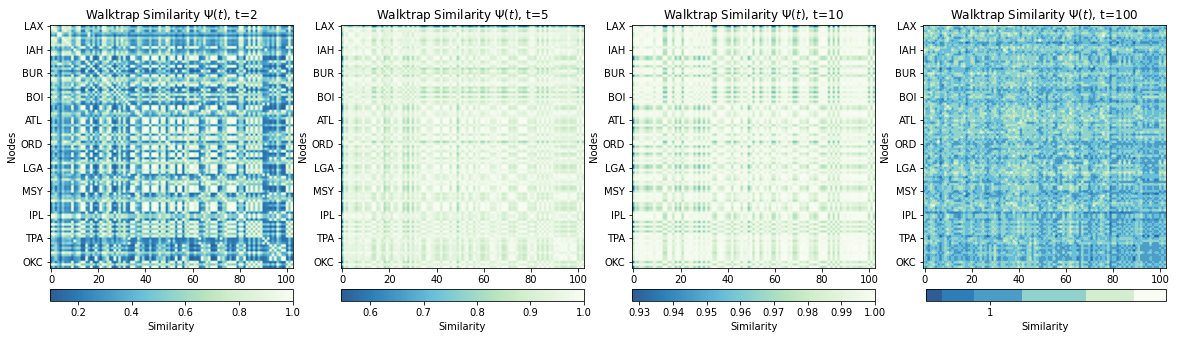
\includegraphics[width=\textwidth]{flight_net/Walktrap_Similarity_flights.png}
    \caption{Walktrap similarity matrices calculated for the flights network.}
    \label{fig:Walktrap flights}
\end{figure}
\begin{figure}[H]
    \centering
    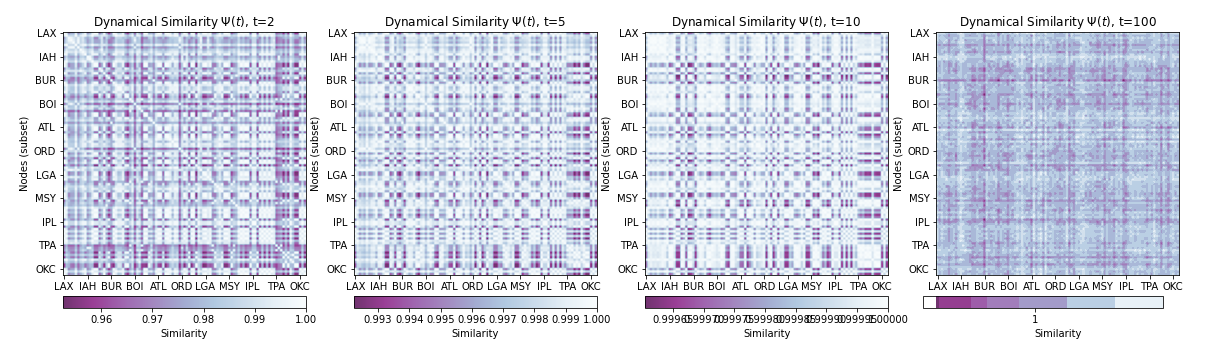
\includegraphics[width=\textwidth]{flight_net/Dynamical_Similarity_flights.png}
    \caption{CTRW dynamical similarity matrices for the flights network.}
    \label{fig:dynamical similarity matrix flights}
\end{figure}
The results of spectral partitioning being performed on these matrices is visualised in Figures \ref{fig:flight predictions t200} and \ref{fig:maps}. (DISCUSS PREDICTIONS HERE).

\begin{figure}[H]
  \begin{subfigure}[b]{0.3\textwidth}
    \centering
    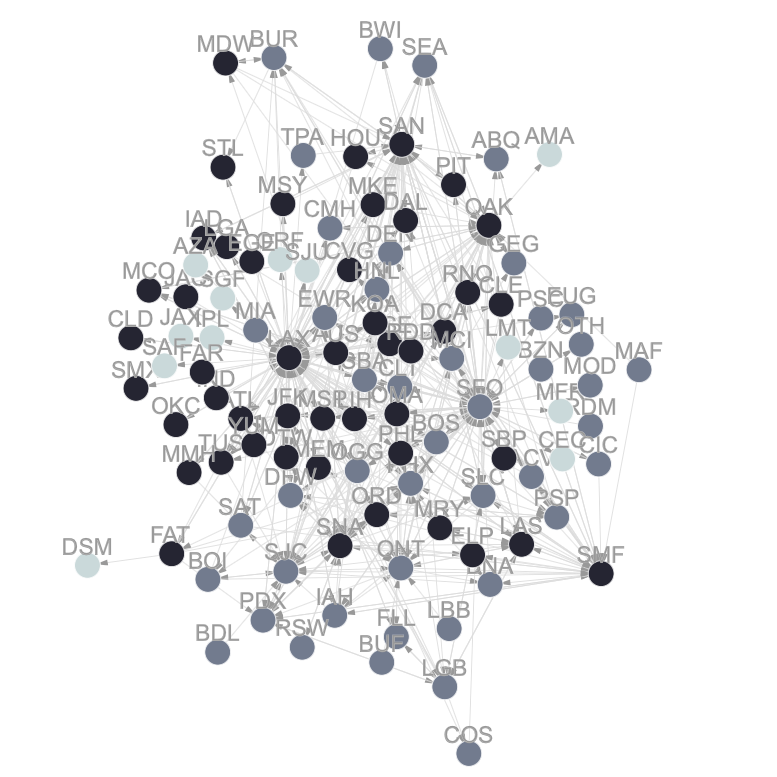
\includegraphics[width=\textwidth]{flight_net/flight partition t100.png}
    \caption{DTRW}
    \label{fig:flights 100 dtrw}
  \end{subfigure}
  \hfill
  \begin{subfigure}[b]{0.3\textwidth}
    \centering
    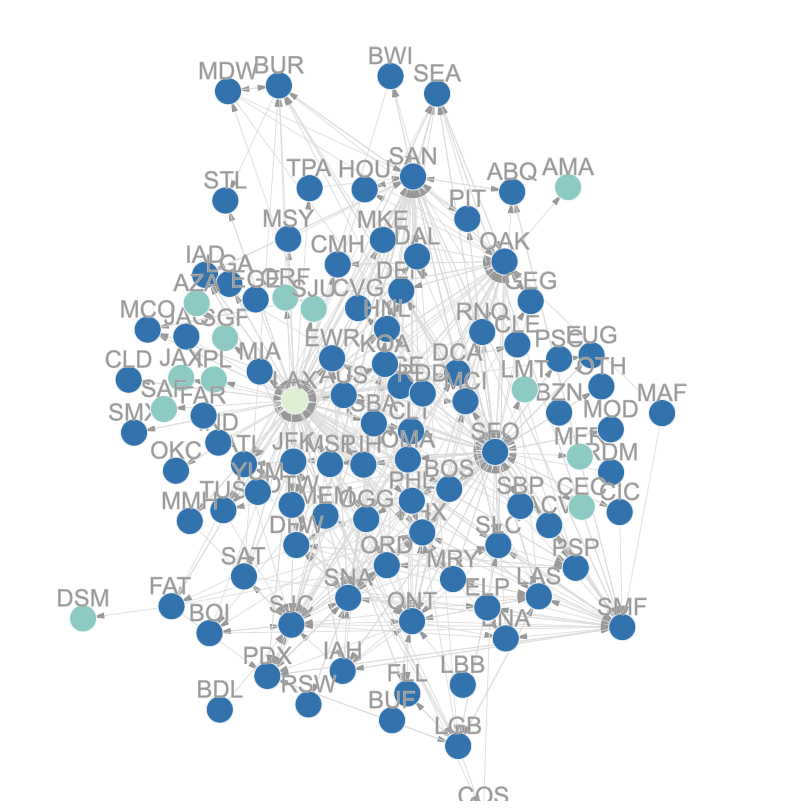
\includegraphics[width=\textwidth]{flight_net/flights partition t100 wt.png}
    \caption{Walktrap}
    \label{fig:flights 100 wt}
  \end{subfigure}
  \hfill
  \begin{subfigure}[b]{0.3\textwidth}
    \centering
    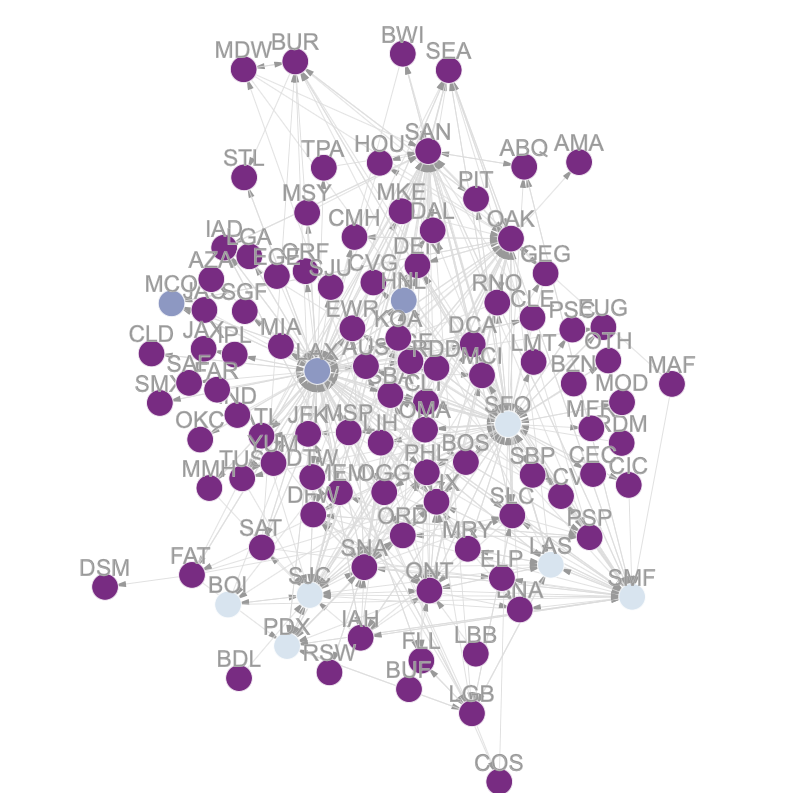
\includegraphics[width=\textwidth]{flight_net/flights partition t100 ctrw.png}
    \caption{CTRW}
    \label{fig:flights 100 dtrw ctrw}
  \end{subfigure}
  \caption{}
  \label{fig:flight predictions t200}
\end{figure}
Flight predictions:

\begin{figure}[H]
  \centering
  \begin{subfigure}[b]{0.5\textwidth}
    \centering
    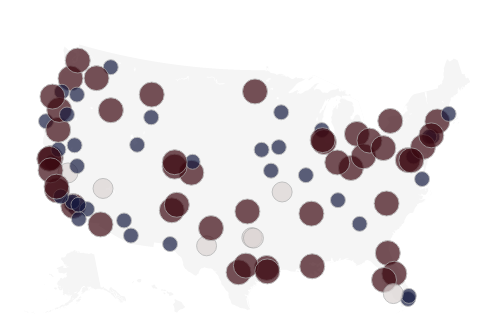
\includegraphics[width=\textwidth]{flight_net/map_DTRW.png}
    \caption{DTRW}
    \label{fig:map_DTRW}
  \end{subfigure}
  \hfill
  \begin{subfigure}[b]{0.5\textwidth}
    \centering
    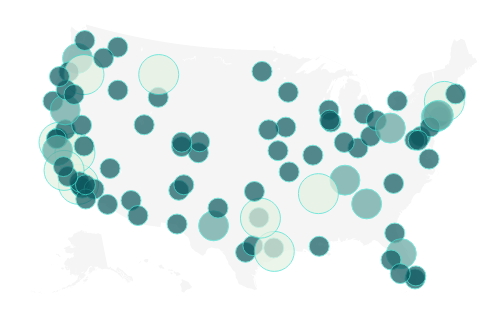
\includegraphics[width=\textwidth]{flight_net/map_wt.png}
    \caption{Walktrap}
    \label{fig:map_wt}
  \end{subfigure}
  \hfill
  \begin{subfigure}[b]{0.5\textwidth}
    \centering
    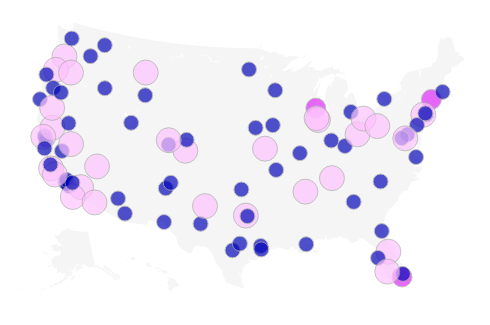
\includegraphics[width=\textwidth]{flight_net/map_dynsim.png}
    \caption{CTRW}
    \label{fig:map_dynsim}
  \end{subfigure}
  \caption{Map visualisations }
  \label{fig:maps}
\end{figure}

\noindent This clustering...

\noindent We now implement generate similarity matrices for time $t=10$, which arguably more realistic of a process that might run on this network where one would expect most passengers to have completed their itineraries within ten flights. The similarity matrices for $t=10$ are still very similar, only varying in the order $\mathcal{O}(10^{-3})$ but the clusters determined my spectral clustering look reasonable. The DTRW-based algorithms group what seem to be more hub-like airports including Los Angeles, San Diego, San Francisco and Oakland into one group. Then the rest of the network appears to be bisected depending on whether the airport is more affiliated with either San Francisco or Los Angeles. \medskip

\noindent The CTRW-based algorithm identifies one cluster that seems to be predominantly Los Angeles and its affiliated airports. The bulk of the other major Californian airports with the exception of maybe San Jose and Sacramento, are then grouped into the second cluster. The third cluster appears to identify slightly less-well integrated airports.

\noindent It is difficult to identify exactly what dynamical similarities have been identified by the algorithms here. There is a strong degree of spatial bias to be expected as networks that are topologically close in the graph will naturally produce similar behaviour in the random walker trajectories, especially when the smaller timescale is used.





%% CORE-PERIPHERY STUFF
\section{Dynamical Core-Periphery Structures}
As mentioned above, the adjacency matrix of the flights network (Fig. \ref{fig:flights adjacency matrix}) is indicative of what is known as a core-periphery structure \cite{kojaku2019multiscale} and indeed, these meso-scale structures have been well-documented and researched in airline networks \cite{kojaku2019multiscale}. For comparison purposes we will perform core-periphery analysis on this network.\\
Core-periphery detection work as follows: align network is partitioned into a group of core nodes, which are strongly connected and a set of peripheral nodes which are weakly connected to that core. The algorithm is DTRW-based and works under the understanding that if a walker is currently at a node that is part of the peripheral group, it's next step is very unlikely to also be in the peripheral group. A walker on a core node, however, is far more likely to remain within the well connected core or return to it quickly if it leaves \cite{lambiottenotes}. To determine the core-periphery structure of a given network at stationarity we first consider planting a walker at the node with the lowest out-strength and call this our initial peripheral set $\mathcal S_0$. If these is more than one node with lowest out-strength then a one of these nodes is chosen randomly. Hence, there is an element of randomness in this algorithm. The persistence probability for a group $\mathcal S$ is defined as the probability that a walker will remain within that group on its next step. For a group consisting of a single node this probability is naturally zero. The measure is defined as \cite{lambiottenotes}
$$\alpha_\mathcal S = \frac{\sum_{i,j \in \mathcal S}\pi_iT_{ij}}{\sum_{i \in \mathcal S}\pi_i} = \frac{\text{Prob\{step to another node in } \mathcal S \text{\}}}{\text{Prob\{step to any other node\}}}$$
where $\pi$ is the stationary probability density of the network and $T$ is the transition matrix defined by $T_{ij} = A_{ij}/s_i^{\text{out}}$.  \\
The algorithm is computationally expensive and works by successively adding the node that least increases the persistence probability to the group $\mathcal S$. As each node is added the amount by which the coreness of $\mathcal S$ increases is recorded and this values is assigned to the node as its coreness value. Finally, a critical $\alpha$-value is decided on and used to make a cut. Nodes with a high coreness value are assigned to the network's core and nodes with coreness below the threshold will be labelled as peripheral.  \medskip

\noindent The algorithm works quite well on the airline network and identifies many of the airports you would expect to be hubs. In particular, it consistenly assigns LAX a far higher coreness score than the other nodes which agrees with the existing perception of LAX as a national and international hub airport \cite{guimera2005worldwide}. The airports with the top five coreness scores are shown in Table \ref{table:coreness}. Other airports regularly classified as core airports include recognisable names such as Las Vegas, Burbank, Phoenix and Oakland. Visuals of the core-periphery grouping are included in Figure \ref{fig:cp viz main}. The random choice element in the algorithm did lead to different groupings and the variation in the coreness score was around $\mathcal{O}(1)$ on different runs. This would be best mitigated by running multiple implementations of the algorithm and taking the average over the coreness scores for each airport (PUT IN CONCLUSION).

\begin{center}
  \csvautotabular{flight_net/top_5_coreness.csv}
  \captionof{table}{Airports with the highest five coreness scores.}
  \label{table:coreness}
\end{center}

\begin{figure}[H]
    \begin{subfigure}[b]{0.5\linewidth}
        \centering
        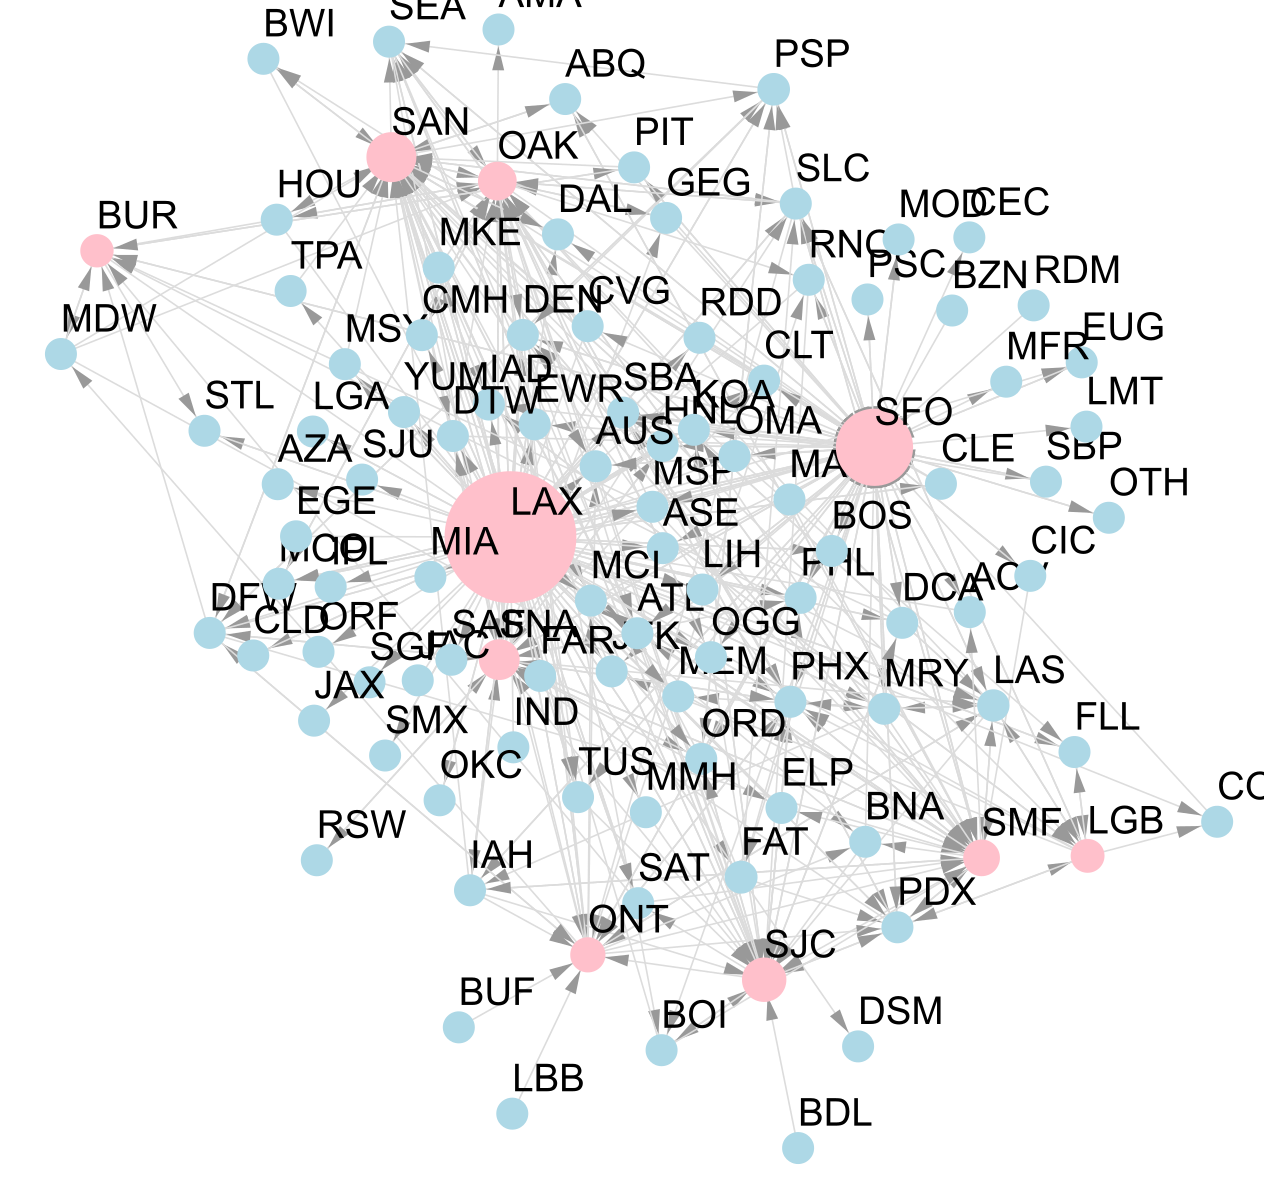
\includegraphics[width=\textwidth]{flight_net/cp_viz.png}
        \caption{}
        \label{fig:cp viz}
    \end{subfigure}
    \begin{subfigure}[b]{0.5\linewidth}
        \centering
        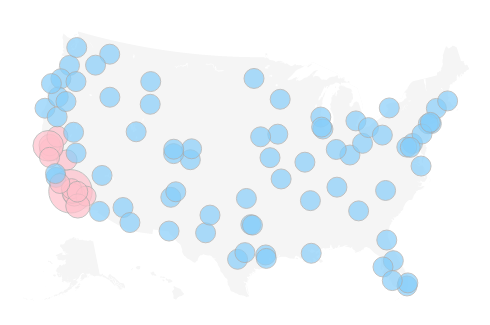
\includegraphics[width=\textwidth]{flight_net/map_coreness.png}
        \caption{}
        \label{fig:map cp}
    \end{subfigure}
    \caption{}
    \label{fig:cp viz main}
\end{figure}

\section{Discussion}
AVERAGING OVER TIMESCALES
\subsection{Memory networks}
Flow-based community detection and node-ranking measures are typically based on the probability paths of a random walker on the network. A walker is injected to a certain node on the network a t$t=0$ and it's probabilities to be at different points of the network evolve with time. This random walker is assumed to have the Markov property, where it goes next depends on on it's current location and it immediately forgets where it was previous to that step. This assumption works well for diffusive dynamics, say, the spreading of \colorbox{yellow}{get example} but has been shown to be a significant oversimplification in many cases \colorbox{yellow}{get ref} such as, for example, in the flow of passengers in air travel where we expect a passengers next destination is highly conditional on where they came from. In these cases, the Markov assumption oversimplifies our understanding of dynamics on a network and valuable information is lost. \colorbox{yellow}{Take about predictive flows}.

\printbibliography
\appendix
\section{Flight clustering results}

\begin{figure}[H]
  \centering
  \begin{subfigure}[b]{0.3\linewidth}
    \centering
  \includesvg[inkscapelatex=false,width=200pt]{dtrw_t10} %fix me
  \caption{}\label{fig:dtrw_t10}
  \end{subfigure}
  \hfill
  \begin{subfigure}[b]{0.3\linewidth}
    \centering
  \includesvg[inkscapelatex=false,width=200pt]{wt_t10} %fix me
  \caption{}\label{fig:wt_t10}
  \end{subfigure}
  \hfill
\end{figure}
\begin{figure}
  \ContinuedFloat
  \begin{subfigure}[b]{0.3\linewidth}
    \centering
  \includesvg[inkscapelatex=false,width=200pt]{dynsim_t10} %fix me
  \caption{}\label{fig:dynsim_t10}
  \end{subfigure}
  \caption{Results of spectral clustering for time $t=10$ and $k=3$ clusters. Figure \ref{dtrw_t10} shows clustering results for the DTRW-based similarity measure, Figure \ref{fig:wt_t10} shows results for the Walktrap-like similarity measure and Figure \ref{fig:dynsim_t10} shows results for the dynamical similarity-based similarity measure.} \label{fig:flights t10}
\end{figure}

\begin{figure}[H]
  \centering
  \begin{subfigure}[b]{0.4\textwidth}
    \centering
    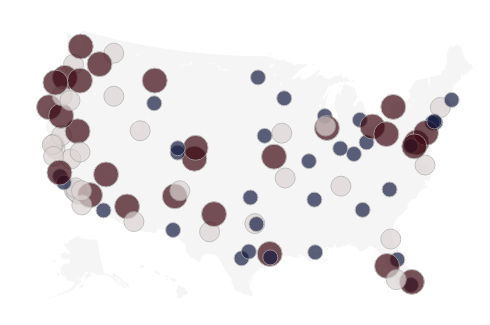
\includegraphics[width=\textwidth]{flight_net/map_DTRW_t10.png}
    \caption{DTRW}
    \label{fig:map_DTRW}
  \end{subfigure}
  \hfill
  \begin{subfigure}[b]{0.4\textwidth}
    \centering
    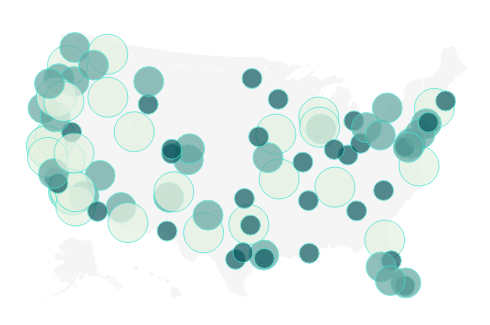
\includegraphics[width=\textwidth]{flight_net/map_wt_t10.png}
    \caption{Walktrap}
    \label{fig:map_wt}
  \end{subfigure}
  \hfill
  \begin{subfigure}[b]{0.4\textwidth}
    \centering
    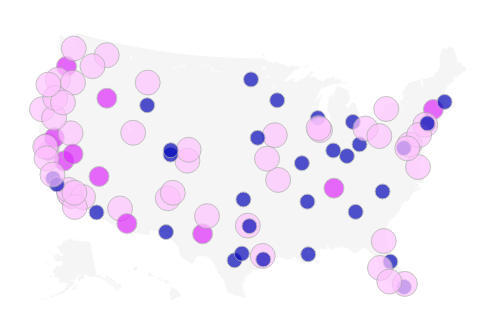
\includegraphics[width=\textwidth]{flight_net/map_dynsim_t10.png}
    \caption{CTRW}
    \label{fig:map_dynsim}
  \end{subfigure}
  \caption{Map visualisations }
  \label{fig:maps}
\end{figure}

\section{Theorems}
(https://stanford.edu/class/ee363/lectures/pf.pdf )
\begin{theorem1}
  If $A$ is a regular matrix, (i.e. $A$ is non-negative and there exists $k>0$ such that $(A^k)_{i j} > 0\, \forall i,j$) then there exists an isolated eigenvalue $\lambda_{\text{pf}}$ of $A$ such that $\lambda_{\text{pf}}$ is positive and $|\lambda|<\lambda_{\text{pf}}$ for all other eigenvalues $\lambda$. Also, the corresponding positive left and right eigenvectors are unique up to positive scaling \cite{boydnotes}.
\end{theorem1}
\begin{theorem2}
  If $A$ is a non-negative and there exists $k>0$ such that $(A^k)_{i j} > 0\, \forall i,j$ then there exists an eigenvalue $\lambda_{\text{pf}}$ of $A$ such that $\lambda_{\text{pf}}$ is positive and $|\lambda|<\lambda_{\text{pf}}$ for all other eigenvalues $\lambda$. Also, the corresponding left and right eigenvectors are nonnegative (but are not necessarily unique or positive) \cite{boydnotes}.
\end{theorem2}



\cite{lambiotte2019networks}
\cite{lambiottenotes}
\end{document}
